\documentclass[main.tex]{subfiles}

\begin{document}
	
\section{Klasifikačné modely}	
Snažili sme sa vybrať binárno-klasifikačné modely a aplikovať ich na úlohu predpovedania, či sa konkrétna politická strana dostane do vlády, alebo nie

\subsection{Výber algoritmov}
Rozhodli sme sa porovnať tieto tri základné algoritmy, ktoré poskytujú rôzne prístupy ku riešeniu tejto klasifikačnej úlohy

\begin{enumerate}
    \item \textbf{Logistická regresia}
    \item \textbf{Rozhodovací strom}
    \item \textbf{Support vector machine}
\end{enumerate}

\subsection{Predspracovanie dát}
Skôr ako sme sa pustili do samotného trénovania týchto modelov, získané dáta sme museli ešte spracovať do \uv{rozumného} formátu.

Dáta o samotných prieskumoch, ktoré sú už vopred rozdelené na trénovaciu a testovaciu vzorku majú takúto štruktúru.

\begin{table}[h!]
    \centering
    \caption{Ukážka dát o prieskumoch}
    \begin{tabular}{llcccl}
        \toprule
        \textbf{political\_party} & \textbf{$\ldots$} & \textbf{elected\_to\_parliament} & \textbf{1} & \textbf{2} & \textbf{$\ldots$} \\
        \midrule
        olano    & $\ldots$ & 0        & 8.2      & 6.4 & $\ldots$ \\
        smer\_sd & $\ldots$ & 1        & 34.6     & 38.4 & $\ldots$ \\
        $\vdots$ & $\vdots$ & $\vdots$ & $\vdots$ & $\vdots$ \\ 
        \bottomrule
    \end{tabular}
\end{table}

Teda máme informácie o názve strany, či bola v danom roku naozaj zvolená alebo nie (hodnota 1 označuje, že bola) a údaj v percentách z prieskumu z $k$ mesiacov pred voľbami, kde $k \in \{ 1, \ldots , 12 \}$. Takisto máme pre každé pozorovanie dátum volieb, informáciu o tom či strana bola predtým v koalícii alebo v opozícii a skutočný percentuálny výsledok volieb v danom roku.

Okrem týchto \uv{hlavných} dát, máme dáta aj dáta \uv{vedľajšie}, ktoré zachytávajú všeobecné informácie o sociálno-ekonomickej situácii na Slovensku v danom roku. 


\begin{table}[h!]
    \centering
    \caption{Ekonomické ukazovatele}
    \begin{tabular}{llcccl}
        \toprule
        \textbf{indicator} & \textbf{2010} & \textbf{2011} & $\ldots$ \\
        \midrule
        Unemployment rate (\%) & 12.46    & 13.59  \\
        GDP (per capita)       & 12668    & 13254 \\
        $\vdots$               & $\vdots$ & $\vdots$ \\ 
        \bottomrule
    \end{tabular}
\end{table}

Tieto dve tabuľky sme na základe rokov spojili a následne zaviedli aj nové premenné, ktoré sú interakciami. Napríklad sme vynásobili binárnu premennú \textit{in\_coallition\_before} s premennou \textit{Unemployment rate} a ešte niektorými premennými zo všeobecných dát.

Nakoniec sme všetky premenné štandardizovali na tzv. \textit{z skóre}, teda každá premenná má priemer 0 a štandardnú odchýlku 1. Z takto znormalizovaných premenných sme vybrali podmnožinu, na ktorej budeme trénovať naše klasifikačné algoritmy. Menovite to boli tieto premenné.

\begin{python}
    final_variables: list[str] = [
        "1", "2", "3", "4", "5", "6", "7", "8", "9", "10", "11", "12",
        "in_coalition_before_Unemployment rate (%)",
        "in_coalition_before_Pension expenditures (per capita)",
        "in_coalition_before_Expenditures on research and development",
        "Risk of poverty rate", "Total household income", "Total inflation rate (%)",
        "Gasoline price 95 octane",
    ]
\end{python}

\subsection{Trieda Ensemble}
Okrem hore-uvedených algoritmov sme naimplementovali aj triedu Ensemble, ktorá spája ľubovolné predikčné algoritmy, ktoré sa podieľajú štýlom \uv{hlasovania} na finálnej predikcii. 
Parametre potrebné na inicializáciu sú tieto.

\begin{python}
    def __init__(self, models: list[Type[BaseEstimator]],
             metric: Callable, threshold: float = 0.5,
             weights: Optional[list[float]] = None) -> None:
\end{python}
\textit{Models} je zoznam modelov, ktoré budú \uv{hlasovať} o finálnej predikcii. Parameter \textit{metric} je metrika na základe ktorej sa  proporčne pridelí každému modelu \uv{sila hlasovania}. Threshold je hyperparameter, ktorý určuje kedy je pozorovanie klasifikované ako \uv{dostane sa do vlády} a kedy nie. Weights je voliteľný parameter, ktorým dopredu môžeme prideliť silu každému modelu.

Po inicializácii môžeme náš \uv{spojený} model natrénovať. Teda trénuje sa osobitne inštancia každého zo vstupných modelov osobitne. Nakoniec sa vypočítajú sily predikcií podľa danej metriky, ktoré sa napokon znormalizujú tak, aby dali v súčte $1$. 

Po úspešnom trénovaní, môžeme predikovať takto.
\begin{python}
    def predict(self, X: pd.DataFrame):
    predictions: list[np.ndarray] = []

    for classifier in self.fitted_classifiers:
        predictions.append(np.array(classifier.predict(X=X)))
    
    weighted_sum: np.ndarray = np.dot(np.array(predictions).T, np.array(self.weights))

    return (weighted_sum >= self.threshold).astype(int)
\end{python}
Vstupom do metódy predict je matica dát a výsledkom je vektor klasifikácii. Po predikcií všetkých modelov sa vypočíta súčin matice predikcií a vektora váh. Nakoniec sa pozložkovo porovná výsledok tohto násobenia so vstupným hyperparametrom \textit{threshold}.

\subsection{Porovnanie algoritmov}

Pre každý z uvedených prístupov nájdeme doprednou selekciou podmnožinu premenných, ktorá nakoniec použijeme pri finálnom natrénovaní. Pre našu triedu \textit{Ensemble} takistou kros-validáciou nájdeme optimálnu hodnotu hyperparametra \textit{threshold} pre túto podmnožinu. Nakoniec už môžme len porovnať tieto natrénové modely na testovacích dátach.

\begin{figure}[!htbp]
    \centering
    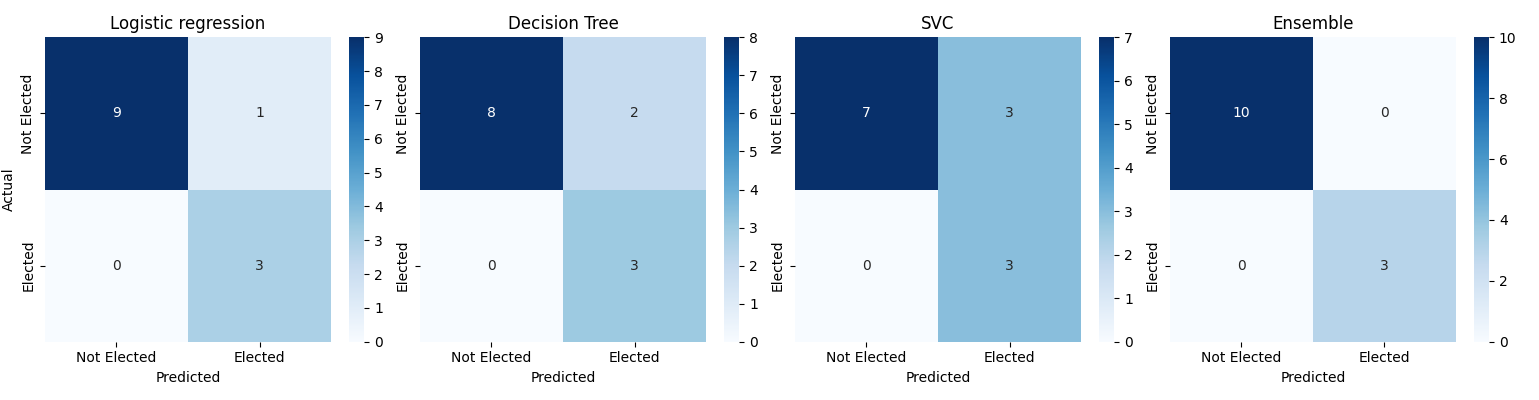
\includegraphics[width=0.98\textwidth]
    {images/confussion_matrix.png}
    \caption{}
    \label{fig:confussion_matrices}
\end{figure}
Môžeme vidieť, že naša trieda, v tomto prípade pozostávajúca práve zo všetkých troch modelov, klasifikovala všetky testovacie dáta správne, narozdiel od modelov samotných, kde boli prípady takzvanej \textit{false positivity}. Hoci sa tento výsledok zdá sľubný, testovacie dáta pozostávali len z trinástich pozorovaní. Otázkou teda zostáva, ako by si naša metóda viedla na väčších dátach.

\end{document}
	